We initially implement the $\phi^4$ model to verify the results of our system. According to previous studies \cite{monahan2016, schaich2006}, the $\phi^4$ model exhibits a symmetric and broken phase depending on its parameters $m_0^2$ and $\lambda$, specifically occurring at $m_0^2 = -0.72$ when $\lambda = 0.5$. We verify this result by plotting four observables: the lattice average $|\langle\bar\phi\rangle|$, the magnetic susceptibility $\chi$, the Binder cumulant $U$ and the bimodality $B$ in Fig.~\ref{fig:phi4}.
\begin{figure}[h]
    \centering
      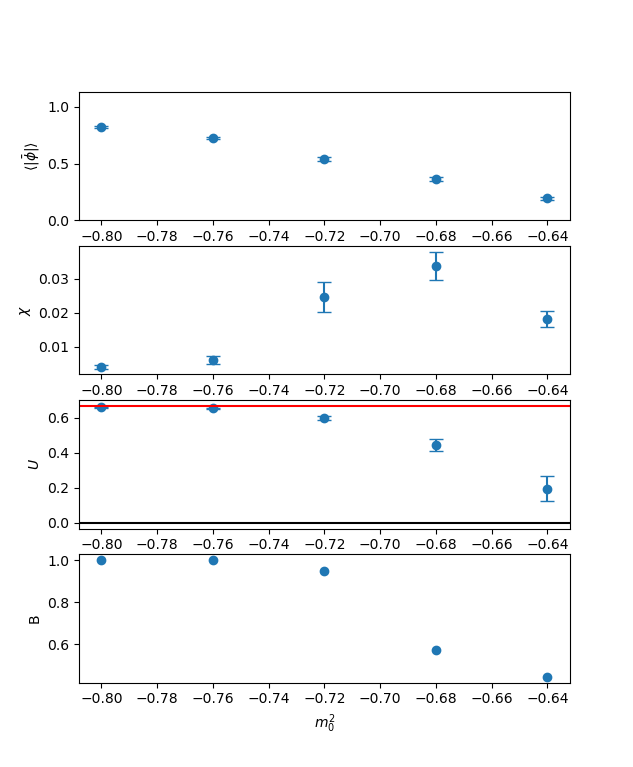
\includegraphics[width=0.7\textwidth]{imgs/phi4.png}
      \caption{\label{fig:phi4} The lattice average $|\langle\bar\phi\rangle|$, the lattice susceptibility $\chi$, the Binder cumulant $U$ and the bimodality $B$ plotted as functions of $m_0^2$. $L=32$, $\lambda=0.5$. The lattice was thermalized from a hot start for 1000 sweeps. Afterwards, 100 measurements were taken with 100 sweeps between each. The red horizontal line indicates $U=2/3$, the symmetric limit of the Binder cumulant.}
\end{figure}
This figure confirms a phase transition near $m_0^2=-0.72$ and supports the accuracy of our model.

\section{Non-linear sigma model results}
After confirming the phase transition in the $\phi^4$ model, we turn to the NLSM. In order to confirm the accuracy of the model, we compare results with existing literature. We first compare our results to Berg \& L\"uscher \cite{berg1981}, specifically measuring the internal energy and magnetic susceptibility. 

\subsection{Comparison with Existing Literature}
Following \cite{berg1981}, we approximate the internal energy in the strong ($\beta<1$) and weak ($\beta>2$) regimes as 
\begin{equation}
    \label{eq:analytic_energy}
E \approx \begin{cases} 
    4-4y-8y^3-\frac{48}{5}y^5& \beta<1 \\
    \frac{2}{\beta} + \frac{4\beta^2} + 0.156\frac{1}{\beta^3}& \beta>2. 
\end{cases}
\end{equation}
We compare this analytical result and simulated values of $\chi_m$ with the Monte Carlo simulation in Fig.~\ref{fig:bergluscher}.
\begin{figure}[h]
    \centering
      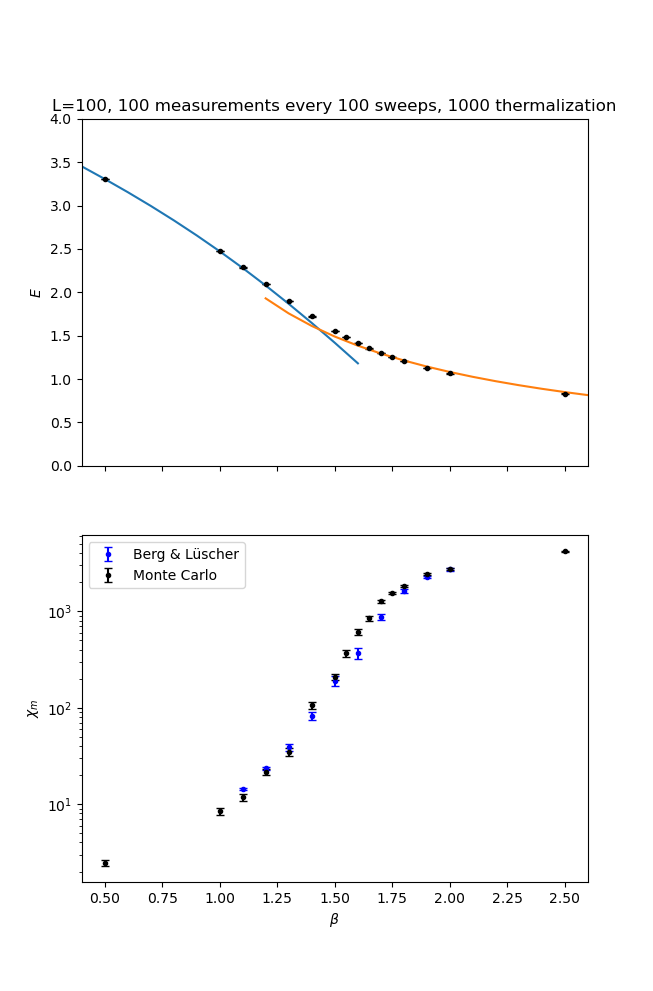
\includegraphics[width=0.6\textwidth]{imgs/internal_energy.png}
      \caption{\label{fig:bergluscher}Comparison with \cite{berg1981}. First panel: internal energy compared with analytic  energy (Eq.~\ref{eq:analytic_energy}). Second panel: magnetic susceptibility compared with literature values.}
\end{figure}
These two charts show a high degree of agreement with the current literature.

We also seek to confirm the results from Bietenholz et al.\cite{bietenholz2018}. Specifically, that the topological susceptibility $\chi_t$ diverges in the continuum limit even at finite flow time. Since $\chi_t$ is in units of inverse distance squared, we multiply by $\xi_2^2$, the square of the second moment correlation length, to achieve a scale-invariant value $\chi_t\xi_2^2$. Additionally, we use a parameter $t_0$ to scale the flow time such that $t_0\sim L^2$. In our Monte Carlo simulation, we adapt the same values as \cite{bietenholz2018} for $\xi_2$.

To begin the comparison, we plot $\chi_t\xi_2^2$ as a function of flow time $\tau$, shown in Fig.~\ref{fig:bietenholz}.
\begin{figure}[h]
    \centering
      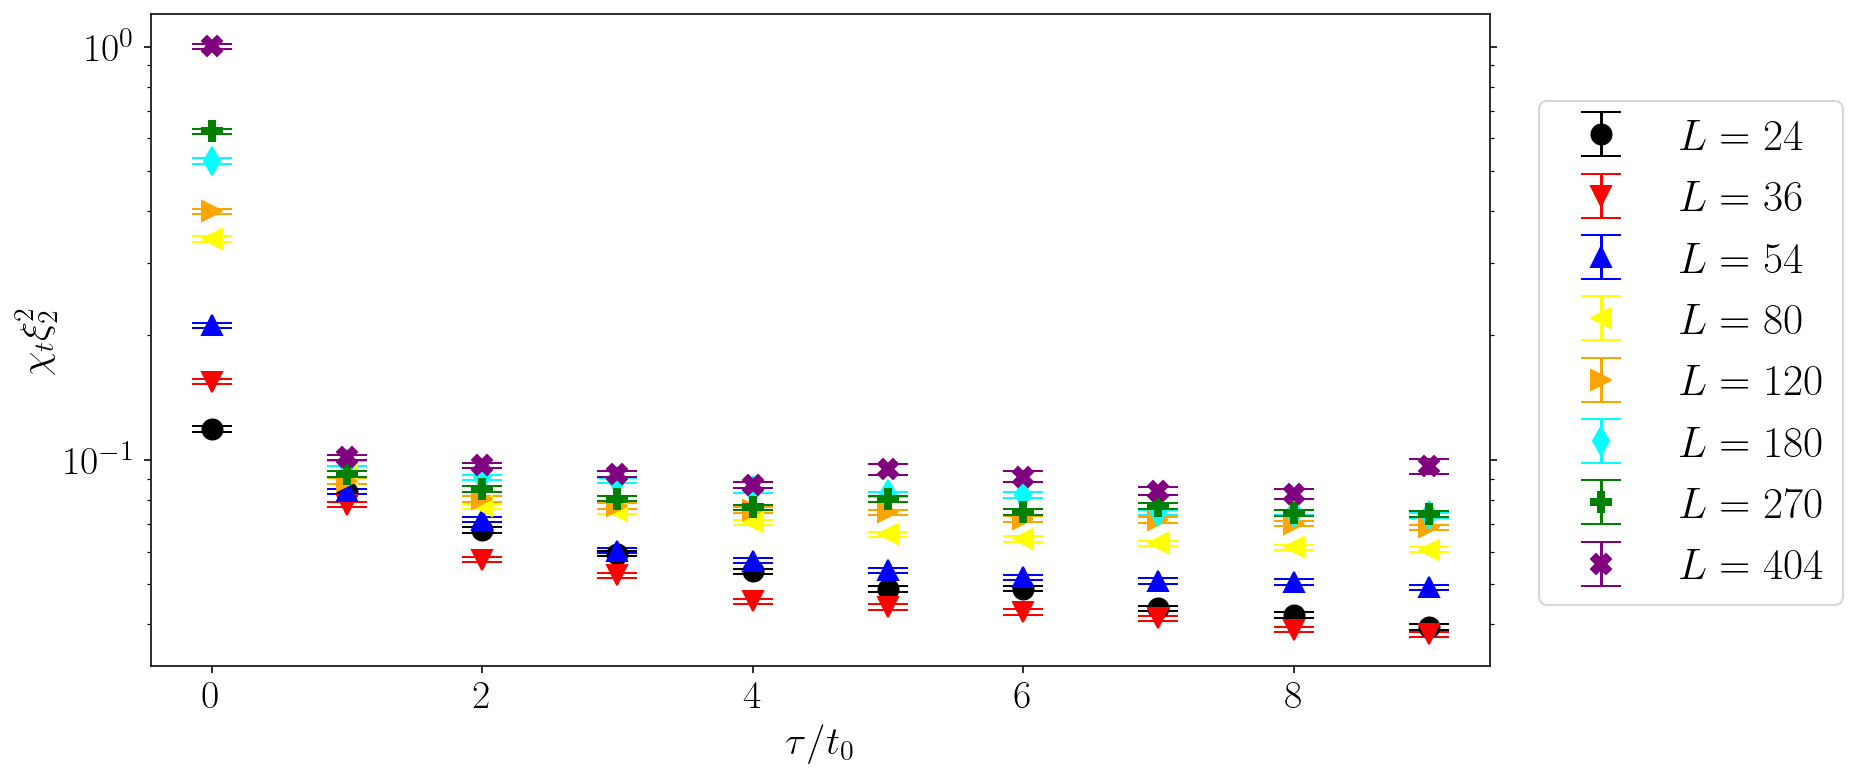
\includegraphics[width=\textwidth]{imgs/bietenholz.png}
      \caption{\label{fig:bietenholz} $\chi_t L^2$ as a  function of flow time $\tau$. Simulation run with 10,000 measurements, measurements very 50 sweeps, 1,000 sweep thermalization.}
\end{figure}
We find that the flow time effectively decreases the topological susceptibility by dampening high-momentum modes. To analyze the divergence of $\chi_t$ in the continuum limit, we plot $\chi_t \xi_2^2$ as a function of lattice size $L$. We perform this simulation at flow time $\tau=5t_0$.
\begin{figure}[h]
    \begin{center}
      \begin{subfigure}[b]{\textwidth}
          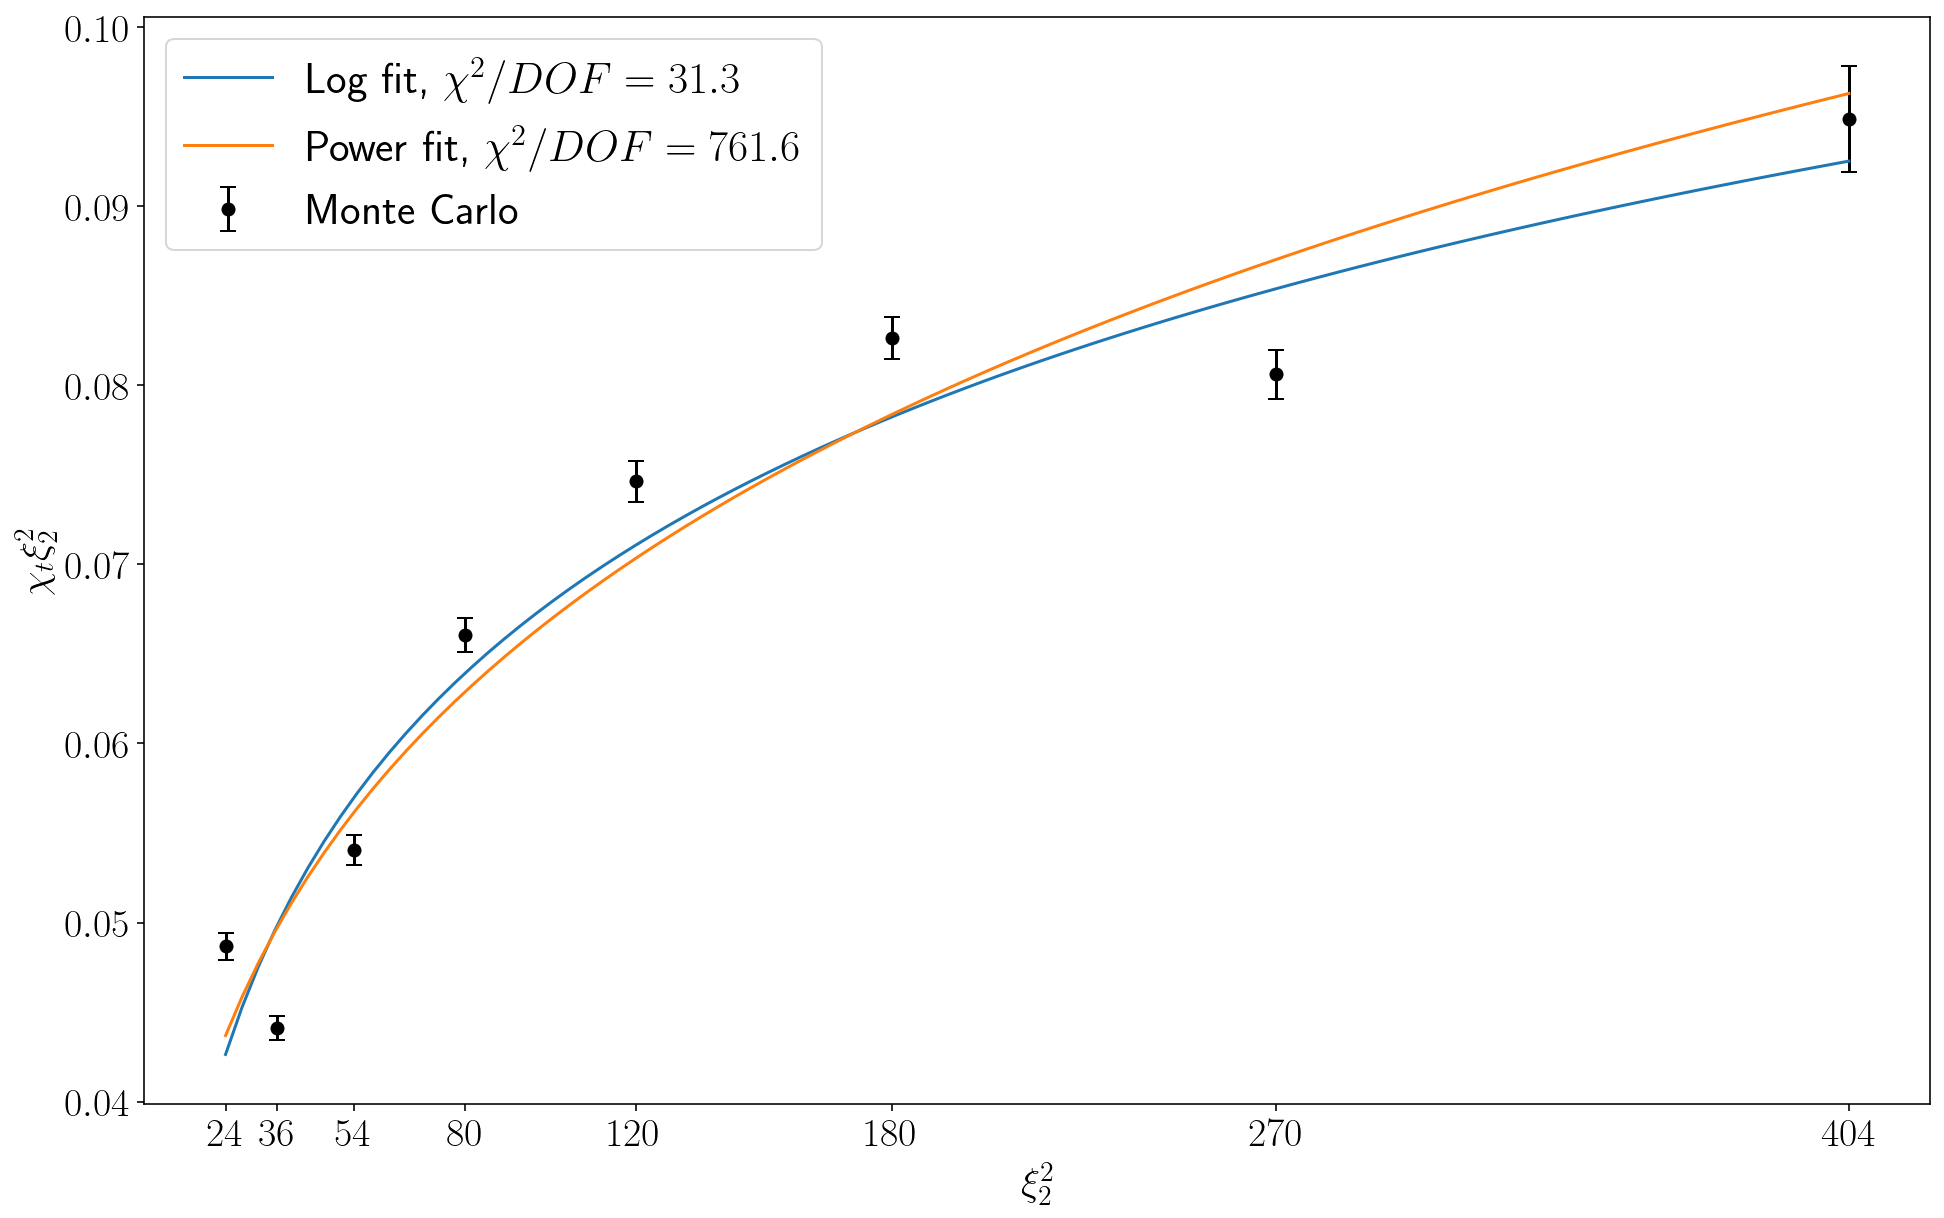
\includegraphics[width=\textwidth]{imgs/divergence.png}
          \caption{$\tau = 0$}
      \end{subfigure}

      \begin{subfigure}[b]{\textwidth}
          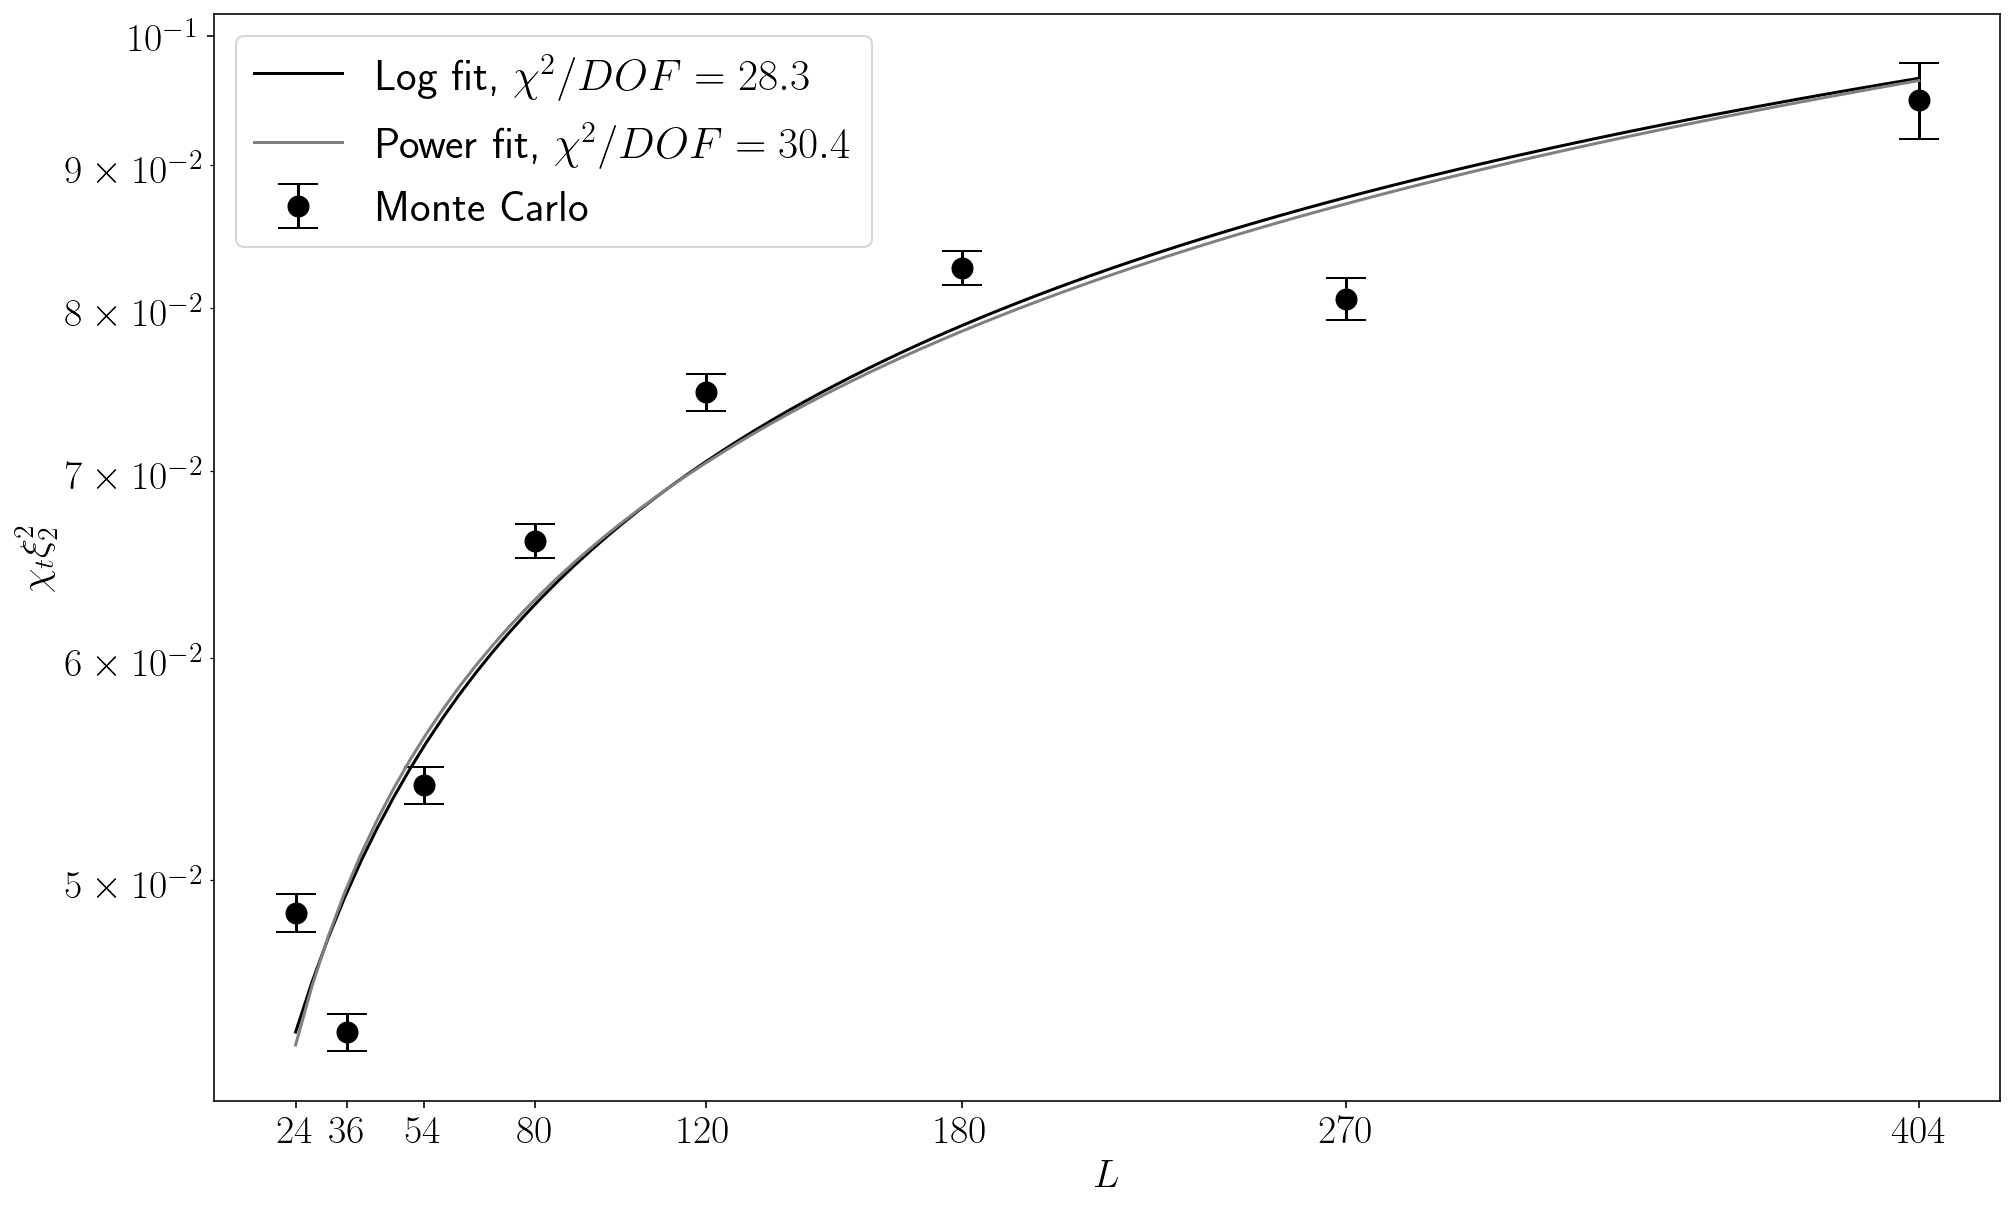
\includegraphics[width=\textwidth]{imgs/divergence_flowed.png}
          \caption{$\tau = 5t_0$}
      \end{subfigure}
      \caption{\label{fig:bietenholz} $\chi_t\xi_2^2$ as a function of $L$. The data is fit with both a log and power fit. Simulation run with 10,000 measurements, measurements very 50 sweeps, 1,000 sweep thermalization. In the $\tau=0$ case, we have compared our result with the curve fit found in \cite{bietenholz2018}.}
    \end{center}
\end{figure}
The data is fit with two options: a log fit
\begin{equation}
    \chi_t \xi_2^2 = A \mathrm{log}(B L) + C
\end{equation}
and a power fit
\begin{equation}
    \chi_t \xi_2^2 = A B^L + C.
\end{equation}
The data fits these functions with $\chi^2/DOF$ of $31.3$ and $761.6$ respectively. Both of these function diverge as $L\rightarrow \infty$, indicating that the topological susceptibility does as well. This is still a slower divergence than the linear divergence featured in the $\tau=0$ case.

\subsection{Topological charge when $\theta\neq 0$}
Following the method explained in Sec.~\ref{sec:topotheta}, we calculate the imaginary part of $\langle Q \rangle$ for arbitrary $\theta$. We perform this calculation for four values of the flow time $\tau$, shown in Fig~\ref{fig:theta}.
\begin{figure}[h]
    \centering
      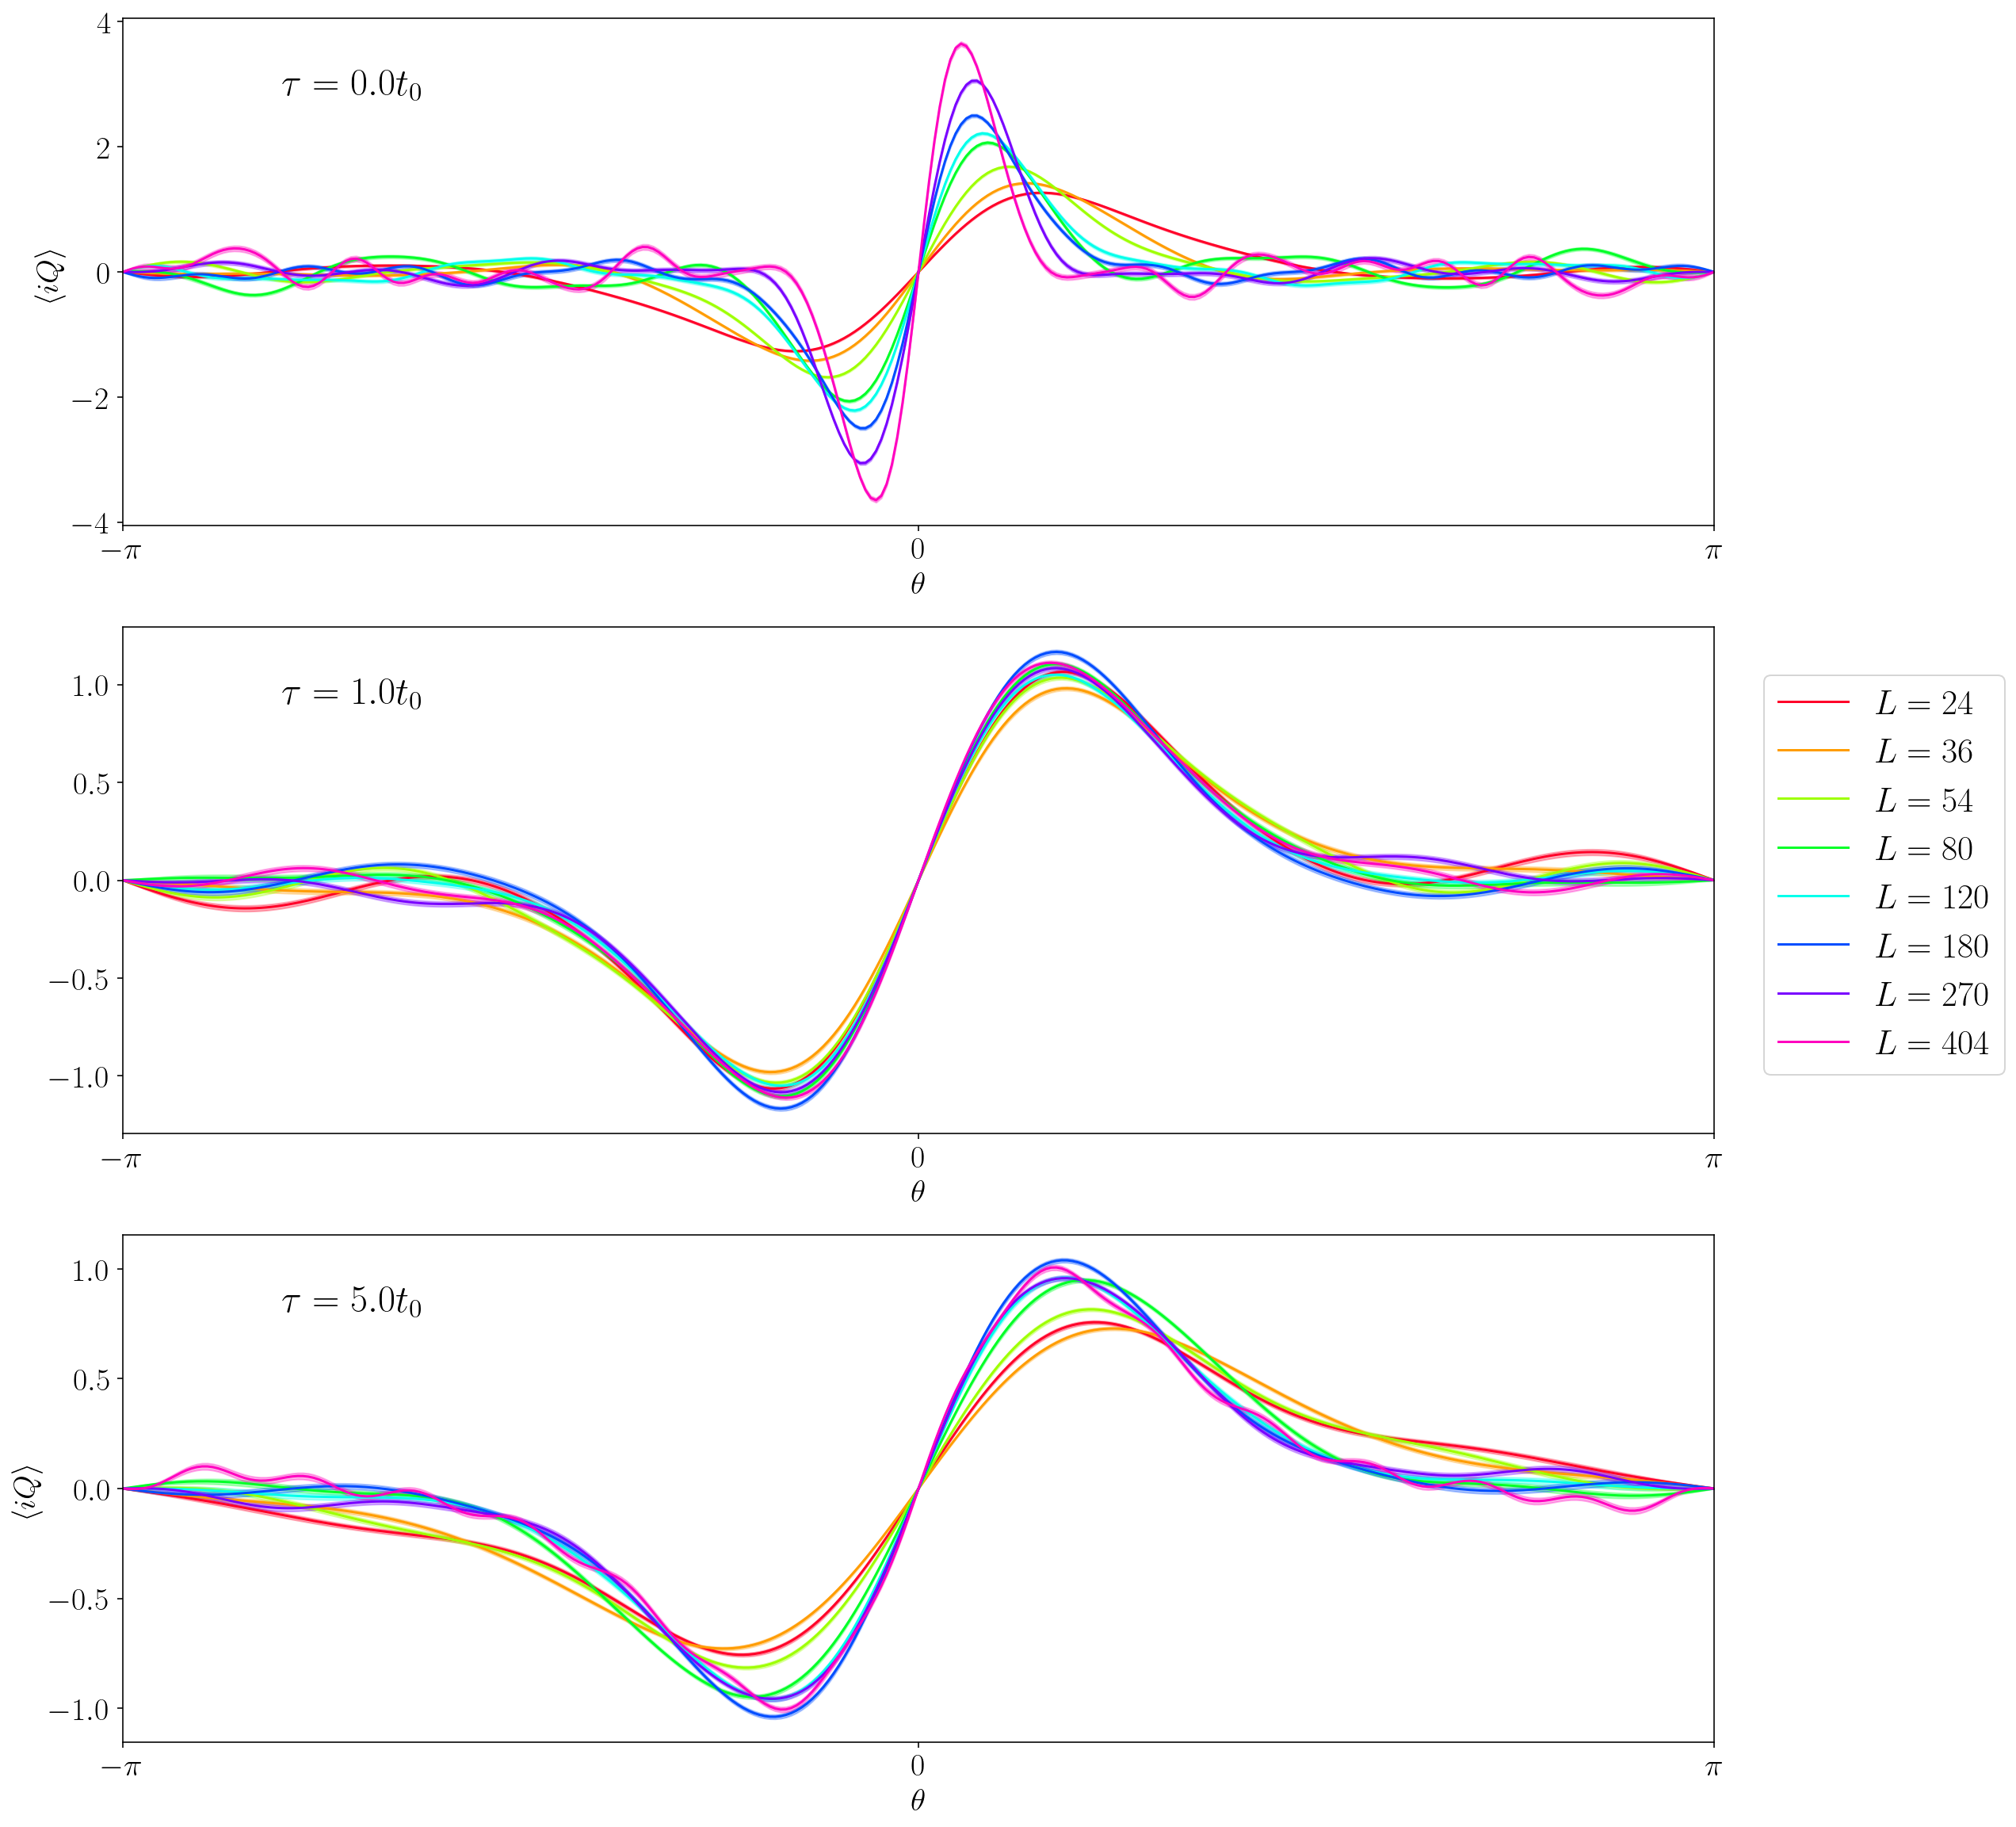
\includegraphics[width=\textwidth]{imgs/theta.png}
      \caption{\label{fig:theta} Imaginary part of $\langle Q \rangle$ as a function of $\theta$. Simulation run with 10,000 measurements, measurements very 50 sweeps, 1,000 sweep thermalization. Note the different scaling of the $y$-axis.}
\end{figure}
These plots demonstrate the divergence of the continuum limit in the $\tau=0$ and the flowed regimes. In the $\tau=0$ case, the slope increases sharply, reflecting the linear divergence of $\chi_t$. However in the flowed regime, this divergence is much slower, reflecting the logarithmic or power-law relationship shown in Fig.~\ref{fig:bietenholz}.

%\chapter{Statistical Analysis}

